\documentclass{beamer}
\usetheme{default}
\usepackage{amsmath,textcomp,amssymb,geometry,graphicx,tabularx,array,hhline,ulem,fancyvrb,upgreek}
\usepackage[export]{adjustbox}
\renewcommand*\arraystretch{1.25}

\title{DREAMER v2\\(Statically Scheduled Logic Emulation)}
\author{Albert Magyar, Richard Lin, Jonathan Bachrach}
\begin{document}

\begin{frame}
\maketitle
\end{frame}

\begin{frame}{Why design a new reconfigurable logic platform?}
\begin{center}
\includegraphics[width=2.8in]{virtex.jpg}
\end{center}
\begin{itemize}
\item Efficient support for word-width operations, debug visibility
\item Enjoy FPGA build times?
\item Enjoy recompiling to change wire visibility with ChipScope?
\end{itemize}
\end{frame}

\begin{frame}{High-level motivation}
\begin{itemize}
\item We want to build a network of small, parallel processors
\item Also supporting tools!
\end{itemize}
\begin{center}
\includegraphics[width=1in]{array_4x4.png}
\end{center}
\begin{itemize}
\item Occupy a new point in the space between programmability and efficiency
\item Explore applications in varied domains
\begin{itemize}
\item Fast logic emulation
\item Providing a new programmable logic target
\item Low-level, low-overhead parallel programming
\end{itemize}
\end{itemize}
\end{frame}

\begin{frame}{Emulation and prototyping}
\begin{center}
\includegraphics[width=1.8in]{chiselator.png}
\end{center}
\begin{itemize}
\item Close designer productivity loop for hardware creation
\begin{itemize}
\item Provide emulation faster than software simulation
\item Provide better dynamic wire visibility than FPGAs
\end{itemize}
\item Fast compile time is a big win here
\begin{itemize}
\item Chisel designs map to the Chiselator in seconds
\item Overall iteration speed much faster 
\end{itemize}
\item Match FPGA in cost
\begin{itemize}
\item Implement array on FPGA for \textit{FPGA overlay}?
\end{itemize}
\end{itemize}
\end{frame}

\begin{frame}{Real implementation target}
\begin{itemize}
\item FPGA alternative
\begin{itemize}
\item Again, beating FPGA tools in compile time is key
\item Hope to beat FPGAs in energy-delay product
\begin{itemize}
\item Multiplex expensive, word-width ALUs in time
\end{itemize}
\end{itemize}
\item Direct programming
\begin{itemize}
\item Highly-parallel execution in dataflow order
\item Is this better than SIMD? {\color{red}For what applications?}
\end{itemize}
\item Maybe an FPGA is the best way to realize this grid $\rightarrow$ \textit{overlay}
\end{itemize}
\begin{center}
\includegraphics[width=2in]{overlay.png}
\end{center}
\end{frame}

\begin{frame}{Array architecture}
\begin{center}
\includegraphics[width=2in]{array_4x4.png}
\end{center}
\begin{itemize}
\item Massively parallel machine (in theory)
\item 4-nearest neighbor connected network
\item Static scheduling of operations and data movement
\item Ready/valid interface on ports $\rightarrow$ supplants noop storage
\item 2-element buffers$\rightarrow$ deadlock less common
\end{itemize}
\end{frame}

\begin{frame}{Tile architecture}
\begin{center}
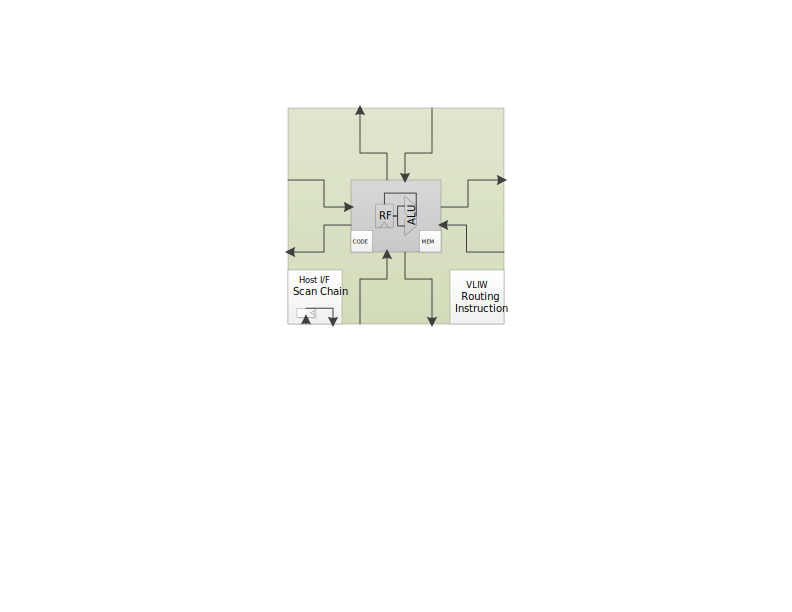
\includegraphics[width=2.5in]{tile.png}
\end{center}
\begin{itemize}
\item Extremely reduced ISA meant for emulation
\item Operations for logical, arithmetic, and mux nodes
\item No branching -- simple emulation loop
\end{itemize}
\end{frame}

\begin{frame}{Initial VLSI results}
\begin{center}
\includegraphics[width=4in]{size_comparisons_array_rocket.png}
\end{center}
\end{frame}

\end{document}